	\subsection{Sensores de Contacto}
\section{Sensores Externos}
\begin{itemize}
	\item \textbf{Interruptores de límite}: El interruptor de límite es un sensor mecánico que se activa al ser presionado, generalmente mediante un brazo mecánico, y puede operar con contacto directo o mediante un imán. Existen en configuraciones normalmente abiertas (NO) y normalmente cerradas (NC), permitiendo o interrumpiendo el flujo de corriente según su activación. También pueden tener uno o varios polos para controlar distintos circuitos. Aunque son fiables, presentan desventajas como desgaste mecánico y menor velocidad en comparación con sensores sin contacto. Se utilizan en robots para detectar posiciones extremas y detener actuadores, evitando daños en la estructura mecánica.
	\begin{figure}[H]
		\centering
		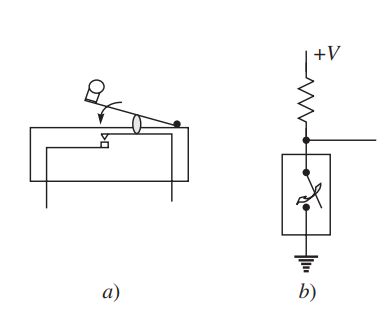
\includegraphics[width=0.5\textwidth]{interruptordelim.png}
		\caption{Interruptor de límite}
	\end{figure}
	
	\item \textbf{Interruptores neumáticos}:Un interruptor neumático es un tipo de dispositivo de conmutación que utiliza aire para funcionar. Cuando se comprime, el interruptor neumático envía un soplo o una bocanada de aire a lo largo de un tubo de PVC hasta un interruptor de aire. El movimiento del aire activará el interruptor de aire, que creará el circuito eléctrico y activará un dispositivo. Los interruptores neumáticos son muy populares y forman parte de nuestra cartera de productos. Debido a que los interruptores neumáticos son necesarios en muchas aplicaciones e industrias.
	\begin{figure}[H]
		\centering
		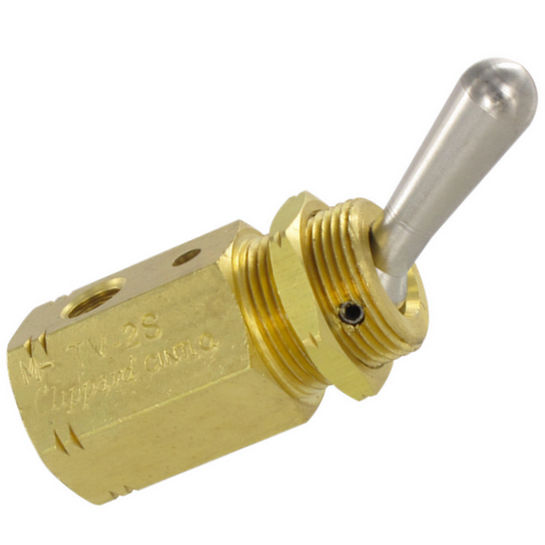
\includegraphics[width=0.35\textwidth]{interruptorneumatico.jpg}
		\caption{Interruptor neumático}
	\end{figure}
	
	
	\item \textbf{Sensores piezoeléctricos}:Un sensor piezoeléctrico es un dispositivo basado en la teoría del efecto piezoeléctrico, el cual es utilizado para medir presión, aceleración, tensión o fuerza; transformando las lecturas en señales eléctricas. Para obtener propiedades piezoeléctricas, el material debe someterse a un fuerte campo eléctrico para secuenciar las cargas. Siendo eliminado el campo eléctrico, la carga se liberará y cuando se aplique presión, la carga se reorganizará para provocar la carga deseada. 
	\begin{figure}[H]
		\centering
		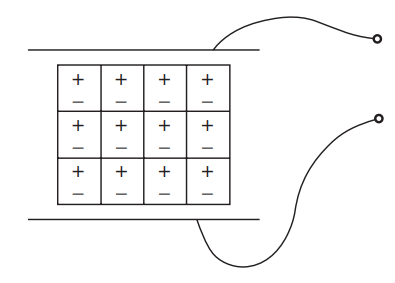
\includegraphics[width=0.5\textwidth]{sensorpiezoelectrico.png}
		\caption{Sensor Piezoeléctrico}
	\end{figure}
	
	\item \textbf{Transductores de presión}:Un transductor de presión convierte la presión en una señal de salida eléctrica. La señal eléctrica puede ser digital o analógica y es utilizada por otros dispositivos como controladores, alarmas y otros sistemas de circuito cerrado. Los transductores de presión se utilizan ampliamente en diversas aplicaciones residenciales y comerciales como bombas, vehículos, aeronaves, etc., donde se requiere la medición de presión. Estos dispositivos son cruciales para garantizar la seguridad y eficiencia en los sistemas al proporcionar datos de presión precisos y en tiempo real.
\end{itemize}
\begin{figure}[H]
	\centering
	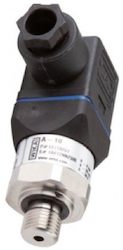
\includegraphics[width=0.125\textwidth]{pressure-transducer.png}
	\caption{Transductor de presión}
\end{figure}

\subsection{Sensores sin Contacto}
\begin{itemize}
	\item \textbf{Sensores de proximidad}: Los sensores de proximidad permiten detectar la presencia o ausencia de objetos sin contacto físico. Se dividen en inductivos y capacitivos.
	\subitem \textbf{ 1.Sensor de proximidad inductivo}: Diseñado para detectar objetos metálicos mediante un campo magnético generado
	por un oscilador.
	\subsubitem -Compuesto por cuatro elementos: bobina y núcleo férrico, circuito oscilador, circuito
	detector y circuito de salida de estado sólido.
	\subsubitem -Funciona detectando cambios en la amplitud del oscilador cuando un objeto entra o
	sale del campo magnético.
	\subsubitem -Tiene un rango de detección típico de 10-15 mm, aunque algunos alcanzan hasta
	100 mm.
	\subsubitem -Factores mecánicos y ambientales pueden afectar su precisión.
	\begin{figure}[H]
		\centering
		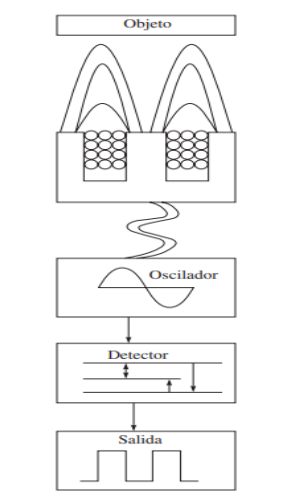
\includegraphics[width=0.3\textwidth]{sensorproxin.png}
		\caption{Sensor de proximidad inductivo} 
	\end{figure}
	\subitem \textbf{ 2.Sensor de proximidad capacitivo}: Similar al inductivo, pero funciona con la capacitancia dieléctrica, permitiendo detectar tanto objetos metálicos como no metálicos.
	\subsubitem -Compuesto por los mismos cuatro elementos del sensor inductivo.
	\subsubitem -Puede detectar objetos ligeros, pequeños y a través de barreras no metálicas (vidrio,plástico).
	\subsubitem - Presenta ventajas como alta velocidad de conmutación, larga vida útil y señal sin rebotes.
	\subsubitem -Limitaciones: afectado por humedad y vaho, y requiere un ajuste de sensibilidad
	para optimizar su rango de detección.
	\subsubitem -Posee mayor alcance que los sensores inductivos y su detección depende del área del plato sensor.
	
	Estos sensores se utilizan ampliamente en la automatización industrial para detectar objetos
	sin contacto, mejorando la eficiencia y precisión en diversas aplicaciones.
	\begin{figure}[H]
		\centering
		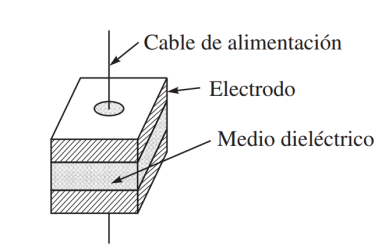
\includegraphics[width=0.4\textwidth]{sensorproxcap.png}
		\caption{Sensor de proximidad capacitivo} 
	\end{figure}
	\item \textbf{Sensores de efecto Hall}: El sensor de efecto Hall es un dispositivo electrónico utilizado para medir campos magnéticos, aprovechando el fenómeno físico conocido como el efecto Hall. Este sensor detecta la presencia, intensidad y dirección de un campo magnético, generando una señal de salida proporcional a la variación del campo. Los sensores de efecto Hall se utilizan principalmente para aplicaciones de posicionamiento, velocidad y control de motores, al detectar la posición de un imán o la rotación de ejes. Son muy útiles en sistemas de retroalimentación, ya que proporcionan una medición precisa sin contacto directo, lo que los hace ideales para entornos en los que se requiere alta fiabilidad y durabilidad. Además, su
	capacidad para operar en condiciones difíciles, como altas temperaturas o ambientes polvorientos, los convierte en una opción valiosa en la automatización y control robótico. 
	\begin{figure}[H]
		\centering
		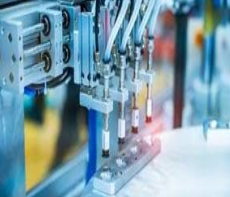
\includegraphics[width=0.4\textwidth]{sensorhallsc.png}
		\caption{Sensor de efecto Hall} 
	\end{figure}
	Ofrecen varias ventajas, como su inmunidad al ruido eléctrico y al polvo, su fiabilidad debido a la ausencia de partes móviles, y su durabilidad gracias a su diseño en estado sólido. Además, son capaces de funcionar en condiciones extremas, sin sufrir rebotes de contacto, lo que les proporciona una larga vida útil. Estos sensores se aplican en áreas como servomotores, sensores de proximidad y velocidad, sistemas de inyección automovilísticos, control de acceso y medición de potencia y campo magnético, siendo esenciales en la
	automatización industrial y el control de movimiento.
	\begin{figure}[H]
		\centering
		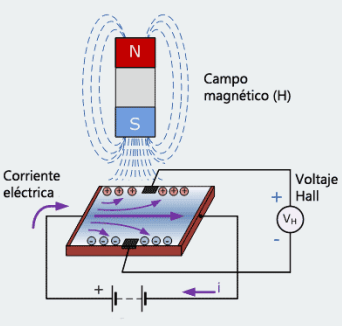
\includegraphics[width=0.4\textwidth]{sefectohall.png}
		\caption{Principios básicos de los sensores de efecto Hall} 
	\end{figure}
	
	\item \textbf{Sensores de microondas}: Los sensores de microondas emplean la frecuencia de microondas para detectar movimiento mediante la emisión de impulsos y el análisis de su reflejo en objetos en movimiento, basándose en el efecto Doppler.
	\begin{figure}[H]
		\centering
		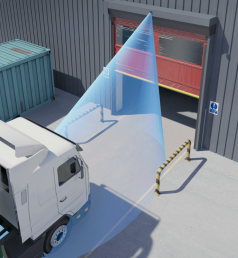
\includegraphics[width=0.4\textwidth]{sensormicroondas.png}
		\caption{Sensor de microondas} 
	\end{figure}
	
	\subitem \textbf{Tipos de Sensores de Microondas}:
	\subsubitem 	1. Radar de Onda Continua (CW): Emite señales continuas y detecta cambios en el
	patrón de reflexión para identificar movimiento.
	\subsubitem 2. Radar de Impulsos: Envía impulsos de microondas y mide el tiempo de retorno para
	determinar la distancia del objeto.
	\subsubitem 3. Radar Doppler: Mide el cambio en la frecuencia de la onda reflejada para detectar
	movimiento.
	\subsubitem 	4. Sensores Biestáticos: Separan la unidad emisora y la receptora, mejorando la
	precisión y reduciendo falsas alarmas.
	\subsubitem 5. Sensores Monostáticos: Integran emisor y receptor en una sola unidad, ofreciendo
	mayor compactación.
	
	Los sensores de microondas son fundamentales en la seguridad perimetral debido a su
	amplia cobertura, lo que los hace ideales para proteger grandes áreas como aeropuertos y
	bases militares. Son efectivos en la reducción de falsas alarmas al diferenciar entre intrusos
	humanos y movimientos de animales o vegetación. Además, funcionan en condiciones
	climáticas adversas como lluvia, niebla o nieve, y se integran con sistemas de CCTV para
	activar grabaciones ante detección de movimiento. Su diseño discreto dificulta su evasión
	por parte de intrusos, y su versatilidad permite combinarlos con otros sistemas de
	seguridad, ofreciendo una protección confiable y efectiva.
	\begin{figure}[H]
		\centering
		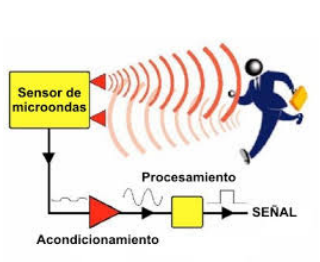
\includegraphics[width=0.4\textwidth]{sensormicro.png}
		\caption{Principios básico de sensores de microondas} 
	\end{figure}
	
	
	
	\item \textbf{Sensores ultrasónicos}: Los sensores ultrasónicos son dispositivos avanzados que utilizan ondas sonoras de alta	frecuencia para detectar objetos y medir distancias con gran precisión. Su función es
	esencial en la robótica, ya que permiten que las máquinas perciban su entorno, facilitando
	una detección confiable y precisa de obstáculos.
	
	La capacidad de detección y evitación de objetos es crucial para la navegación y operación
	eficiente de los robots, especialmente en aplicaciones críticas como vehículos autónomos y
	robots médicos. Sin estos sistemas, los robots podrían enfrentar dificultades para reconocer
	su entorno, lo que podría generar accidentes o fallos en su desempeño. Para mejorar estas
	capacidades, los ingenieros emplean tecnologías avanzadas como visión por computadora,
	aprendizaje automático y sensores ultrasónicos, optimizando así la seguridad, eficiencia y
	automatización en diversas industrias. Los sensores ultrasónicos, como el HC-SR04,
	funcionan emitiendo ondas sonoras de alta frecuencia que rebotan en los objetos,
	permitiendo calcular con precisión la distancia. Son especialmente útiles en entornos
	desafiantes, como áreas con polvo o humo, donde otros sensores pueden fallar. Sin
	embargo, pueden experimentar interferencias, que se resuelven mediante técnicas como el
	salto de frecuencia.
	\begin{figure}[H]
		\centering
		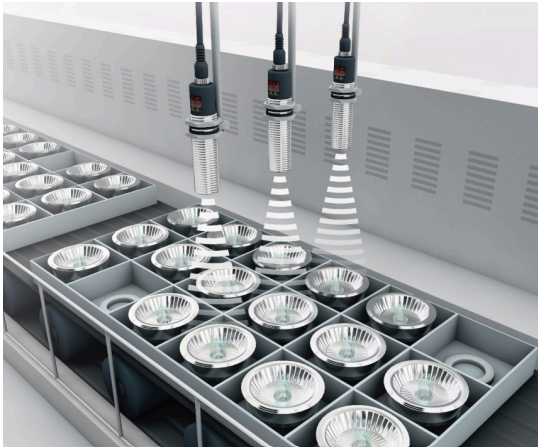
\includegraphics[width=0.4\textwidth]{sultra.png}
		\caption{Sensor Ultrasónico} 
	\end{figure}
	Cálculo de distancia con sensores ultrasónicos:
	
	El sensor ultrasónico mide la distancia de un objeto mediante la siguiente fórmula:
	
	Distancia = (Tiempo de eco x Velocidad del sonido en el aire) / 2
	
	Este método garantiza mediciones exactas y es especialmente útil en entornos donde otros
	sensores, como los infrarrojos, pueden no ser efectivos.
	\begin{figure}[H]
		\centering
		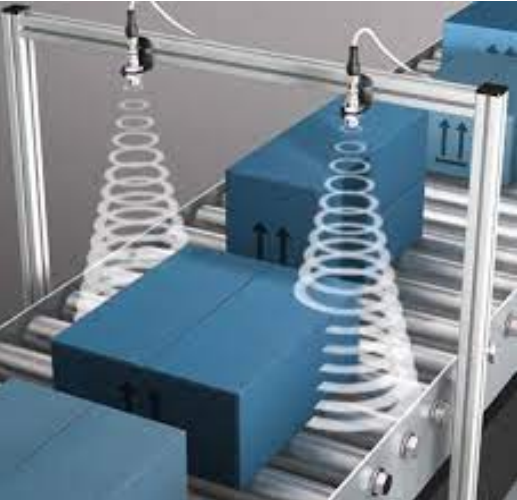
\includegraphics[width=0.4\textwidth]{sensorultra.png}
		\caption{Sensor Ultrasónico} 
	\end{figure}
	
	\item \textbf{Sensores láser}: Un sensor láser es un dispositivo que utiliza tecnología láser para medir distancias, detectar objetos o mapear entornos. Funciona emitiendo un haz de luz láser que se refleja en los
	objetos cercanos y regresa al sensor, lo que permite calcular la distancia entre el sensor y el
	objeto mediante el tiempo que tarda la luz en regresar. Los sensores láser son ampliamente
	utilizados en aplicaciones como la navegación autónoma de robots, mapeo en 3D,
	detección de obstáculos y sistemas de localización. Su alta precisión y capacidad para
	operar en entornos complejos los hacen esenciales en la robótica avanzada, especialmente
	en robots móviles y vehículos autónomos.
	\begin{figure}[H]
		\centering
		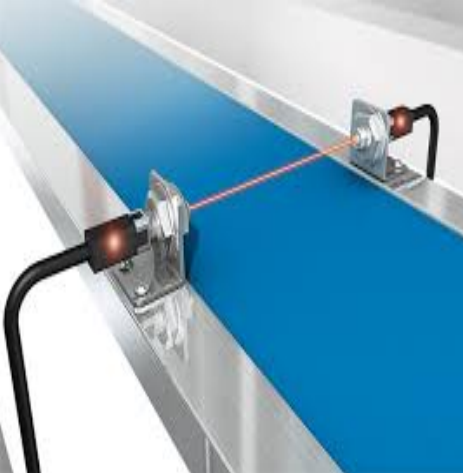
\includegraphics[width=0.4\textwidth]{sensorlaser.png}
		\caption{Sensor láser} 
	\end{figure}
	
	Los láseres son ampliamente utilizados en robótica, especialmente en sensores de
	medición láser. Su implementación permite a los robots lograr un posicionamiento, control y
	detección de seguridad de alta precisión, lo que contribuye significativamente a mejorar la
	productividad y la calidad del producto
	
	
	\item \textbf{Sensores de visión}: Un sensor de visión es un dispositivo tecnológico utilizado para capturar imágenes y procesarlas, con el objetivo de interpretar información visual en el entorno de un sistema o
	robot. Estos sensores funcionan mediante cámaras o sistemas ópticos avanzados que
	analizan imágenes y extraen datos relevantes, como la forma, el color, la posición o el
	movimiento de los objetos en su campo de visión. Son fundamentales para tareas como la
	inspección, la detección de fallos, la navegación autónoma y la manipulación precisa de
	objetos, mejorando la flexibilidad, precisión y eficiencia en sistemas automatizados y robots.
	\begin{figure}[H]
		\centering
		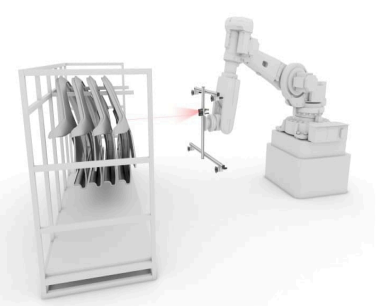
\includegraphics[width=0.4\textwidth]{sensordevis.png}
		\caption{Sensor de visión} 
	\end{figure}
	
	Los sensores de visión están diseñados para adaptarse a diversas variaciones ambientales,
	permitiendo su uso en celdas preconfiguradas sin la necesidad de ajustes costosos. Entre
	sus funcionalidades destacan el aumento de la flexibilidad, la posibilidad de ejecutar
	múltiples tipos de inspección en una sola imagen, la generación de datos detallados para
	mejorar la calidad y los procesos, y la capacidad de ajustarse a desalineaciones en el
	manejo de objetos. Entre sus principales beneficios se incluye la identificación de
	características difíciles de detectar por otros sensores, mejorando el brillo, contraste e
	iluminación de las imágenes a través de filtros y sistemas de iluminación ajustables, y
	gestionando desalineaciones e irregularidades sin importar la velocidad o posición de los
	objetos. Además, su configuración y programación son más sencillas gracias a las
	comunicaciones integradas por Ethernet, lo que facilita la comunicación de los resultados
	con otros sistemas.
	\begin{figure}[H]
		\centering
		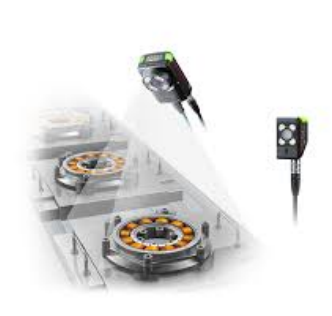
\includegraphics[width=0.4\textwidth]{sensorvision.png}
		\caption{Sensor de visión} 
	\end{figure}
\end{itemize}